\documentclass[landscape,a4paper]{cheatsheet}
\usepackage[ngerman]{babel}
\usepackage[utf8]{inputenc}
\usepackage{float}
\usepackage{graphics}

\title{\texttt{Git} for gits}
\author{A. C. Hinrichs}
\date{\today}

\newcommand{\highlight}[1]{{\textsf{\color{primaryColor}#1}}}
\begin{document}
\maketitle

\begin{figure}[H]
  \centering
  \resizebox{0.75\linewidth}{!}{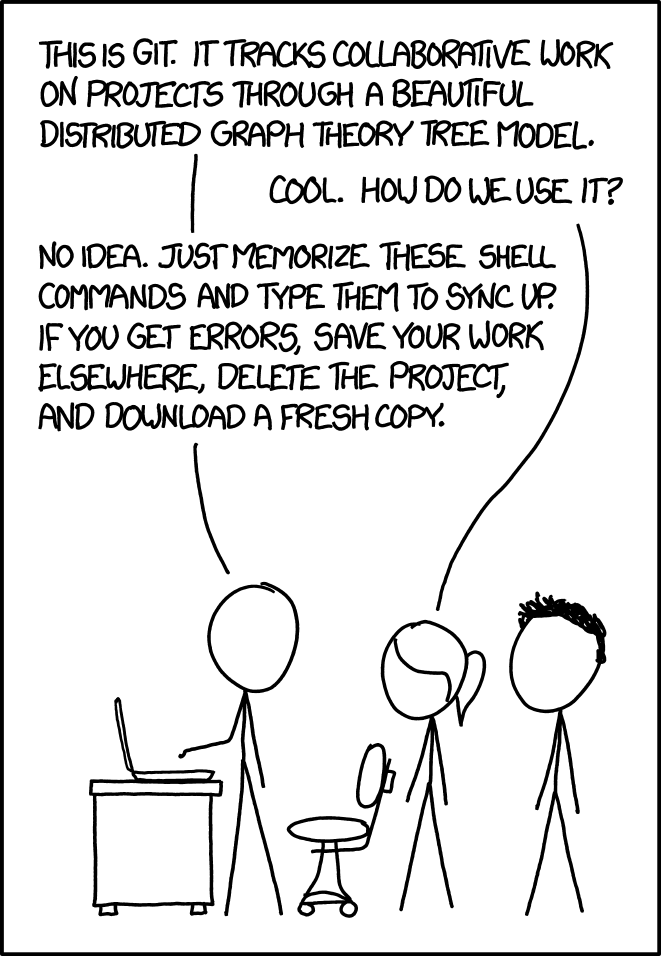
\includegraphics{pictures/git_2x.png}}
  \caption{Anleitung für diese Anleitung\protect\footnotemark}
  \label{fig:anleitung}
\end{figure}
\footnotetext{Quelle: \url{https://xkcd.com/1597/}}
\section{Basis-Workflow}
Ein generischer Git-workflow, ein \highlight{Repository} muss
logischerweise nur ein mal angelegt werden, 
\subsection{Ein \highlight{Repository} klonen}
\begin{lstlisting}[language=bash]
  $ git clone <REPO-URL>
\end{lstlisting} % $ %Hack for Math-highlighting
Git erstelt nun eine \highlight{Arbeitskopie} des entferneten
Repos. Diese liegt anschließend in einem Unterorder des aktiven
Verzeichnisses. 

Exisitert kein entferntes Repository kann man das aktive
verzeichniss mittels
\begin{lstlisting}[language=bash]
  $ git init
\end{lstlisting} % $ %Hack for Math-highlighting
als Repository intialisieren.
\subsection{Einen \highlight{Branch} erstellen \& auf ihn wechseln}
Die Entwicklung auf zwei verschiedenen Branches verläuft komplett
unabhöngig voneinander
\begin{lstlisting}[language=bash]
  $ git checkout -b <NEW-BRANCHNAME>
\end{lstlisting} % $ %Hack for Math-highlighting
Wenn der Branch bereits existiert, kann die Option \lstinline{-b}
weggelassen werden.

Alle (lokalen) Branches kann man sich mit dem Befehl
\begin{lstlisting}[language=bash]
  $ git branch --list
\end{lstlisting} % $ %Hack for Math-highlighting
anzeigen lassen.
\subsection{Im Repository Arbeiten}
Wie auf einer nicht Versionierter Code-Base.

Ist das Arbeitsverzeichniss im Vergleich zum letzen Commit verändert,
so sagt man dass es \highlight{dirty}  also Schmutzig ist.
\subsection{Änderungen \highlight{Commiten}}
Die geänderten Dateien kann man sich mit dem Befehl 
\begin{lstlisting}[language=bash]
  $ git status
\end{lstlisting} % $ %Hack for Math-highlighting
ausgeben lassen.

Um seine Änderungen zum \highlight{Index} hinzuzufügen (also dafür zu
sorgen, dass Git sie sich merkt) nutzt man folgendes Kommando
\begin{lstlisting}[language=bash]
  $ git add <FILENAME>
\end{lstlisting} % $ %Hack for Math-highlighting
Dies funktioniert auch für Verzeichnisse. Gibt man als Dateinamen
\lstinline{.} an, so legt Git alle Änderungen auf den Index.

Man erstellt nun einen \highlight{Commit} mit dem Befehl 
\begin{lstlisting}[language=bash]
  $ git commit -m <COMMIT-NACHRICHT>
\end{lstlisting} % $ %Hack for Math-highlighting

\subsection{\highlight{Pushen} und \highlight{Pullen}}
Um Änderungen aus dem entfernten Repository zu laden:
\begin{lstlisting}[language=bash]
  $ git pull
\end{lstlisting} % $ %Hack for Math-highlighting

Um seine Commits auf das entfernte Repo zu laden:
\begin{lstlisting}[language=bash]
  $ git push
\end{lstlisting} % $ %Hack for Math-highlighting

\subsection{\highlight{Mergen}}
Git ist sehr gut darin, Änderungen zusammenzuführen, benötigt aber
manchmal dabei Hilfe (Git wird einen darauf hinweise). Diese
\highlight{Merge Konflikte} lassen sich mittels dem tool
\begin{lstlisting}[language=bash]
  $ git mergetool
\end{lstlisting} % $ %Hack for Math-highlighting
zusammenführen. Ich empfehle immer die Option
\lstinline{--tool=emerge} anzugeben\footnote{um seinen Merge mit dem
  besten Editor durchzuführen}.

\subsection{Branche zusammenführen}
Auch verschiedene Branches werden \enquote{gemerged}:
\begin{lstlisting}[language=bash]
  $ git checkout <ZIEL BRANCH>
  $ git merge <QUELL BRANCH>
\end{lstlisting} % $ %Hack for Math-highlighting
Merged den Branch \lstinline{<QUELL BRANCH>} in den Branch
\lstinline{<ZIEL BRANCH>}
\end{document}